\documentclass{article}
\usepackage{hyperref}   % For clickable links
\usepackage{fancyhdr}   % For headers and footers
\usepackage{geometry}   % For page margins
\usepackage{graphicx}   % For images
\usepackage{enumitem}   % For better lists
\usepackage{titlesec}
\geometry{a4paper, margin=1in}

% Input variables from external file
% Metadata
\newcommand{\ProjectName}{SORNgen}
\newcommand{\Version}{v1.2.8}
\newcommand{\DocVersion}{v1.0}
\newcommand{\MainRepo}{https://github.com/Maloxoc/sorngen\_2}
\newcommand{\hrefRepo}{\url{\MainRepo}}
\newcommand{\License}{\href{https://github.com/Maloxoc/sorngen_2/blob/main/LICENSE}{LICENSE}}

% Maintainer
\newcommand{\Maintainer}{Jochen Rust}
\newcommand{\MaintainerEmail}{Jochen.Rust@haw-hamburg.de}
\newcommand{\MailToMaintainer}{\href{mailto:\MaintainerEmail}{\MaintainerEmail}}
\newcommand{\MaintainerGitHub}{https://github.com/JochenRust}
\newcommand{\MaintainerGitHubHandle}{@JochenRust}

% Developer
\newcommand{\Developer}{Marvin Henkel}
\newcommand{\DeveloperEmail}{Marvin.Henkel@haw-hamburg.de}
\newcommand{\MailToDeveloper}{\href{mailto:\DeveloperEmail}{\DeveloperEmail}}
\newcommand{\DeveloperGitHub}{https://github.com/Maloxoc}
\newcommand{\DeveloperGitHubHandle}{@Maloxoc}
\newcommand{\parv}[1]{\vspace{#1}}
\newcommand{\parvh}[2]{\vspace{#1} \hspace{#2}}

\newcommand{\newpar}{\parv{8pt}}
\newcommand{\newparind}{\parvh{4pt}{16pt}}

\newcommand{\command}[1]{
\begin{center}
\newpar #1 \newpar
\end{center}
}
\newcommand{\needed}[1]{\textless#1\textgreater}
\newcommand{\optional}[1]{[#1]}

% global settings
\setlength{\parindent}{0pt}
\setlist[enumerate]{label*=\arabic*.}
\graphicspath{ {./images/} }

% Title and author information
\title{\textbf{\ProjectName}}
\author{Marvin Henkel}
\date{01.10.2024}


% Custom header and footer
\pagestyle{fancy}
\fancyhf{}
\fancyhead[L]{\ProjectName\ \Version}
\fancyhead[R]{Version \DocVersion}
\fancyfoot[C]{\thepage}

\begin{document}

% Title page
\maketitle

\section*{Version}
\begin{tabular}{ll}
\textbf{Project Version:} & \Version \\
\textbf{Documentation Version:} & \DocVersion
\end{tabular}

\section*{Overview}
\textbf{\ProjectName} is a python-based tool to generate VHDL code for arithmetic algorithms processed in SORN arithmetic. 

SORN (set of real numbers) is a datatype related to type-2 unum format. For more information see \url{http://www.johngustafson.net/pubs/RadicalApproach.pdf}

This documentation (in its current state) is just containing the sorngen GUI. For information regarding the base project contact Jochen.Rust@haw-hamburg.de

\section*{Contact}
\begin{tabular}{ll}
\textbf{Maintainer:} & \Maintainer \\
\textbf{Email:} & \MailToMaintainer \\
\textbf{GitHub:} & \href{\MaintainerGitHub}{\MaintainerGitHubHandle}\\
\\
\textbf{Developer (GUI):} & \Developer \\
\textbf{Email:} & \MailToDeveloper \\
\textbf{GitHub:} & \href{\DeveloperGitHub}{\DeveloperGitHubHandle}
\end{tabular}

\section*{Additional Resources}
\textbf{Project Repository: } \hrefRepo


\newpage

\tableofcontents

\newpage

% Sections in the document

\section{Installation}
\label{sec:installation}
In order to install \ProjectName, download the project from \hrefRepo. 
If you have Git installed, you can also run the following command:

\command{git clone \MainRepo}
This will download the project into your current working directory.

\newpar Additionally, an installation of Python 3.* is required. You can download it from \url{https://www.python.org/downloads/} (recommended version: 3.12.3)

Lastly, you have to install numpy. To do so, execute the following command in a command prompt:

\command{pip3 install numpy}

\newpage
\section{Getting Started}
\label{sec:getting_started}

\subsection{Starting the tool}
The \ProjectName-tool is available in the sorngen.py file. To launch the GUI, please refer to section \ref{ter:starting_gui}.

Since the project is organized as a Python module, you need to start it using the '-m' switch from a command line interface (CLI) or a similar environment. Additionally, you must provide the path to a specification file (see \ref{ter:spec_file}). Assuming your current working directory is set to the project root (which contains the playground, stable and documentation directories), you can execute the following command:

\command{python -m stable.sorngen \needed{specification file}}

If the specification file is valid, the tool will generate VHDL code in the current working directory. To specify a different output directory, simply append the desired path:

\command{python -m stable.sorngen \needed{specification file} \optional{output directory}}

Regardless of where the output directory is located, a 'VHDL' folder will be created, and the generated code will be placed inside.

\subsection{The specification file}
\label{ter:spec_file}
The specification file is crucial, as it defines the type of module(s) the tool will generate. Understanding the structure and contents of this file is essential for effectively using \ProjectName.

The specification file has a '.sorn' ending and contains all information about name, datatype, pipeline registers and the integrated equations of your Hardware design.

\begin{itemize}
    \item Name: Set the name of the design. The toplevel VHDL file will be "[name].vhd".
    \item Datatype: ['lin'/'log'/'man', '[start,stop,step]', 'zero', 'negative', 'infinity']
    \begin{itemize}
        \item 'lin'/'log': choose either a linear or logarithmic spacing of the lattice values
        \item 'man': choose a fully manually defined datatype
        \begin{itemize}
            \item define datatype as ['man','{<interval1>;<interval2>;<...>}'] with <interval> having open "(" and closed "[" interval bounds
            \item see "MIMO\_solver\_N2" inside the "stable/templates" directory for an example
        \end{itemize}
        \item '[start,stop,step]': choose the start and end value for the lattice values and a stepsize for a linear scale 
        \item 'zero', 'negative', 'infinity': extend the datatype by the given options (any combination can be choosen)
    \end{itemize}
    \item Pipeline registers: The amount of specified registers will be inserted in the design.
    \item Equations: Specify one or multiple equations with consistent variable names, round brackets and python-based arithmetic operators. Variables may appear in multiple equations.
    \item Examples: See the files "MIMO\_solver\_N2.sorn" and "MIMO\_solver\_N4.sorn" inside the "stable/templates" directory.
\end{itemize}

\subsection{The GUI} 
\label{ter:starting_gui}
To launch the graphical user interface (GUI) of the \ProjectName-tool, use the 'App.py' file.
Just like starting the tool via the command line, the GUI must be launched using the '-m' switch. Assuming your current working directory is the project root, run the following command:

\command{python -m stable.App}

This will open the GUI, where you can input the specification (see \ref{ter:spec_file}) in the main text area. If you have an existing specification file, you can load it using the "Open Specification" button at the top of the window.

Once the hardware behavior is defined in the specification, proceed to the next design step by pressing the "Next Step" button. If an error occurs during any design step, it will be highlighted in the upper-right section.

When a design step completes successfully, a confirmation will also appear in the top-right section, and the interface will transition to the next design step screen. As of now, only the specification phase is implemented, so subsequent steps will display a "Not Implemented" message. Future versions will include detailed information on the processing status of the input data during these stages.

To the right of the main panel, additional details and potential issues about the current design step will be displayed. You can also review the log of the entire process by clicking the "Open Log" button in the lower-right corner. This log contains all outputs generated by the script up to that point.

You can revisit previous design steps by selecting the buttons on the left side of the window. If you want to regenerate the output for a specific step—such as after modifying the specification—you can do so by pressing the "Regenerate" button in the lower-left corner. Keep in mind, if you make changes to the specification, you will need to regenerate the output for all subsequent steps.

If you prefer to execute all steps in sequence without reviewing each individually, click the "Run All Steps" button.

Additionally, you can save and load your project at any time using the "Save Project" and "Open Project" buttons located in the upper-left corner. Projects are saved as .sorngen files. Important: Never open untrusted .sorngen files, as they may contain malicious code.

\newpage
\section{Developer Guide}
\label{sec:developer_guide}

\subsection{General Information}
The base \ProjectName-tool is based on the Paper "\href{https://www.researchgate.net/publication/340244525_A_Hardware_Generator_for_SORN_Arithmetic}{A Hardware Generator for SORN Arithmetic}" (especially Section III. "The Hardware Generator"). While the paper contains some outdated information, it still outlines the general architecture and functionality of the tool.

The tool is written entirely in Python, so a basic understanding of Python is recommended. To ensure easier refactoring and scalability, the project follows the Python package structure.
\subsection{The GUI Structure}
\subsubsection{General Architecture}
\label{ter:general_architecture}
The GUI was developed using python 3.12.3 and is implemented using the built-in \href{https://docs.python.org/3/library/tkinter.html}{tkinter} package.

The interface layout currently uses the grid layout manager (see resource \ref{fig:root_layout}) to allow for flexible positioning of widgets. However, it may be beneficial to switch to a different layout manager, like stacking frames side by side, instead of directly positioning widgets within the root.

For details regarding the grid layout manager, refer to \url{https://www.pythonguis.com/tutorials/create-ui-with-tkinter-grid-layout-manager/}

The sections (as seen in resource \ref{fig:root_map}) are named as follows:

\label{enum:root_map}
\begin{enumerate}
    \item main\_frame: Placeholder for the content frames (see Section \ref{ter:main_frames})
    \item project\_frame: Hosts buttons for project management.
    \item windows\_frame: Contains tabs for switching between different content areas in the main frame.
    \item navigation\_frame: Hosts navigation buttons for design flow steps.
    \item status\_frame: Displays the current status of each design step.
    \item info\_frame: Displays quick log messages or information generated during the design process.
    \item This area has no specific name but contains the toggle button for the console.
\end{enumerate}
\subsubsection{Main Frames}
\label{ter:main_frames}
Main frames display critical information for the current or previous design flow steps. Every step (except for the final code generation) has its own dedicated frame:
\begin{enumerate}
    \item specification\_frame: A text field for entering specifications.
    \item parsing\_frame: Displays parsing information (currently not implemented).
    \item elaboration\_frame: Displays elaboration information (currently not implemented).
    \item architecture\_frame: Displays architecture information (currently not implemented).
    \item sorn\_op\_frame: Displays information about SORN operations (currently not implemented).
    \item console\_frame: Contains the log field.
\end{enumerate}

The switch\_to(tk.Frame) method can change the currently displayed main frame. Since it applies layout configurations to the new frame, any tk.Frame object can become a main frame. These frames are generated via the gui.components script (see Section \ref{ter:new_content})

\subsubsection{Surrounding/ Meta Frames}
The surrounding Frames around the main frame are mostly static tk.Frame objects containing different buttons and labels. They are already describe in \ref{enum:root_map} (from 2).
They are generated using the gui.components script (see \ref{ter:new_content} for more information)

\subsubsection{STD Handler}
To capture and manage all output from the script, the class gui.aux\_lib.std\_handler is used. You can start capturing output with the capture method, and stop with the stop method.

\subsection{Adding new content}
\label{ter:new_content}
The gui.components script contains useful methods for adding new widgets.

\subsubsection{Versioning}
For compatibility and error tracking between different project versions, a simple version control number is implemented (see control.version). This version must be manually updated. Although it has no automatic effect, it's recommended to update the version with each addition or modification.

\subsubsection{Frames}
To create new tk.Frame objects, use the gui.components.get\_frame function. The required input is a root widget, which can be any tkinter widget (e.g., tk.Frame). Optional parameters include:
\begin{itemize}
    \item bg: str, background color.
    \item row, col: int: grid layout positions for the widget.
    \item rowspan, colspan: int, span of rows/columns.
    \item sticky: str, directions to stick (north, south, east, west).
    \item padx, pady: int/ tuple[int, int], padding around the widget.
    \item render: bool, whether to render the widget (default is true).
    \item border: bool, if set to true, the frame will have a border.
\end{itemize}

To add a title bar to a frame, use the add\_title\_frame method, specifying the frame and the title (as a tk.StringVar object). Optionally, you can add buttons to the title bar by passing a list of tuples (label, function).

This method will push all containing elements of a tk.Frame one row lower and add a title bar with your specified title and if given buttons.

\subsubsection{Buttons}
Buttons are created using the get\_button method, which essentially works the same as get\_frame. In addition to the root widget, you must provide a name and a callable function for the button. Some optional arguments (e.g., render and border) are not available for buttons.

\subsubsection{Text Fields} % + Log-Field + STD-Handler
For text fields, use the get\_text\_field method, specifying the root widget and optional background color and padding. The two types of text fields are:
\begin{itemize}
    \item tk.Text objects, created using get\_text\_field.
    \item Log fields, a subclass of tk.Text, created using get\_log\_field. Log fields are used to record script outputs. To append to the log, use the log method. If you created the Log field via get\_log\_field, you can add a severity to the log method ("info", "warning", "error", "success")
\end{itemize}

\subsubsection{Canvas}
Although a get\_canvas method exists, it currently generates a placeholder canvas that displays "not implemented."

\subsubsection{Labels}
There are two types of labels:
\begin{itemize}
    \item Regular labels, created with the get\_label method.
    \item Status labels, created with get\_status\_label. Status labels are specialized for displaying statuses ("idle", "running", "success", "failure") and should be managed via their methods, not directly modified.
\end{itemize}

\subsection{Localisation}
\label{ter:localisation}
\subsubsection{How it works}
The current localisation system, implemented in the gui.localisation.translator.Translator class, is essentially a lightweight, dictionary-based solution. During the setup process, the class generates a tk.StringVar object for each key in the default (initial) language.

At the moment, only English is supported. However, if additional languages are available, the translate(str) method can be used to switch the language. This method will update all tk.StringVar objects to the desired translation automatically. To retrieve a tk.StringVar object, call the get(str) method with the corresponding key. This will return a reference to the tk.StringVar object, so any future calls to translate(str) will update the object dynamically.

For cases where a key has multiple meanings (e.g., a toggle button that switches between "open log" and "close log"), the set\_to(str, str) method can be used. This requires two arguments:
\begin{enumerate}
    \item The key of the tk.StringVar object you want to modify.
    \item An additional key that references the specific value within the first key.
\end{enumerate}

Essentially, this acts as a nested dictionary structure, where a single key can have multiple sub-keys to handle context-specific translations.

\subsubsection{How to add new languages}
To add a new language, follow these steps:
\begin{enumerate}
    \item Create a new language script in the gui/localisation directory. For simplicity, it is recommended to copy an existing language script (e.g., the English file) and rename it.
    \item Manually translate each value in the file.
\end{enumerate}

Once the new language script is ready, add it to the get\_dict(str) function. A basic language script follows this structure (see gui.localisation.english for reference):

\command{translations = \{
    $<key_1>: <translation_1>, 
    ... 
    <key_n>: <translation_n>$
\}}


\subsubsection{How to add new keys}
The current localisation system requires each new key to be added manually to every language file. If a key has a single meaning, you can assign it directly to the desired translation. For keys that handle multiple meanings (such as toggle states), you can assign a nested dictionary with sub-keys and corresponding translations.

The structure for multiple meanings looks like this:

\command{$<key> : \{
    <subkey_1>: subtranslation_1,
    ...
    <subkey_n>: subtranslation_n$
\}}

During the initialisation process, the first sub-translation will be selected by default. For examples of this structure, refer to the gui.localisation.english file.

\newpage
\section{Roadmap}
\label{sec:roadmap}
\subsection{Design-flow-step Frames}
As mentioned in section \ref{ter:starting_gui}, not all design-flow-step frames have been implemented yet. The remaining frames to be added include:
\begin{enumerate}
    \item The Parsing Frame
    \item The Elaboration Frame
    \item The Architecture Frame
    \item The SORN operations Frame
\end{enumerate}
These Frames should contain and give information about the current phase of the data processing. The intended contents of each frame are as follows:
\begin{center}
    \begin{tabular}{rl}
        Parsing Frame: & Displays the Abstract Syntax Tree (AST) \\
        Elaboration Frame: & Displays the SORN Syntax Tree (SST) \\
        Architecture Frame: & Shows HDL Diagrams \\
        SORN operations Frame: & Displays the relevant SORN Intervals
    \end{tabular}
\end{center}

\textbf{\large Implementation Notes:}

The first three frames (Parsing, Elaboration, and Architecture) will likely use Canvas widgets to render trees and diagrams directly, potentially based on XML data. In contrast, the SORN Operations Frame will likely involve a table-based representation. Since Tkinter does not provide a native table widget, a custom table will need to be implemented.

Additionally, simply adding these frames to the GUI will not be sufficient; the underlying data structures need to be handled efficiently. This includes modifying the current saving and loading mechanisms to support storing and retrieving information specific to each frame.

While some of this information is currently available in the log as text, visualizing it more intuitively will be crucial for troubleshooting and improving usability.

The following resources may be helpful when implementing these features:
\begin{itemize}
    \item \url{https://tkdocs.com/tutorial/canvas.html}
    \item \url{https://stackoverflow.com/questions/9348264/does-tkinter-have-a-table-widget}
    \item \url{https://www.geeksforgeeks.org/create-table-using-tkinter/}
\end{itemize}

\subsection{Optimisation}
While the current framework performs adequately, certain sections of the code may require refactoring and optimization, particularly when handling larger specifications. Although no major performance issues have been identified, minor slowdowns could occur with more complex inputs. Therefore, ongoing optimization is recommended to ensure scalability and efficiency.

Additionally, as stated in \ref{ter:general_architecture}, it is recommended to switch from using the grid layout manager to a different layout manager, firstly because the grid layout manager may be prone to errors (on this scale of layout) and because it makes adding new content more difficult.

\subsection{Localisation}
\label{ter:roadmap_localisation}
As mentioned in Section\ref{ter:localisation}the current implementation of localisation is quite basic. Adding a new language requires creating a new language script that mirrors every key present in the existing language scripts, and then incorporating this script into the translator.

While this process is relatively straightforward, it becomes more error-prone when adding new keys (e.g., for new features). Each new key must be added manually to every language script, which increases the risk of missing or inconsistent translations.

To mitigate these issues, it is recommended to enhance the localisation system. Potential improvements include:
\begin{itemize}
    \item Implementing a base language that the translator can fall back on if a key is missing in another language script.
    \item Centralizing all keys in a single, unified script to simplify management.
    \item Using .yml or .json formats for the language files instead of Python scripts, as these formats are more widely used for localisation and are easier to maintain.
\end{itemize}

By making these improvements, the localisation system would become more scalable, easier to manage, and less error-prone.

\newpage
\section{License}
\label{sec:license}
This project is licensed under the MIT License - see the \License\ file for details.

\newpage
\section{Resources}
\label{sec:resources}

\begin{figure}[h]
    \centering
    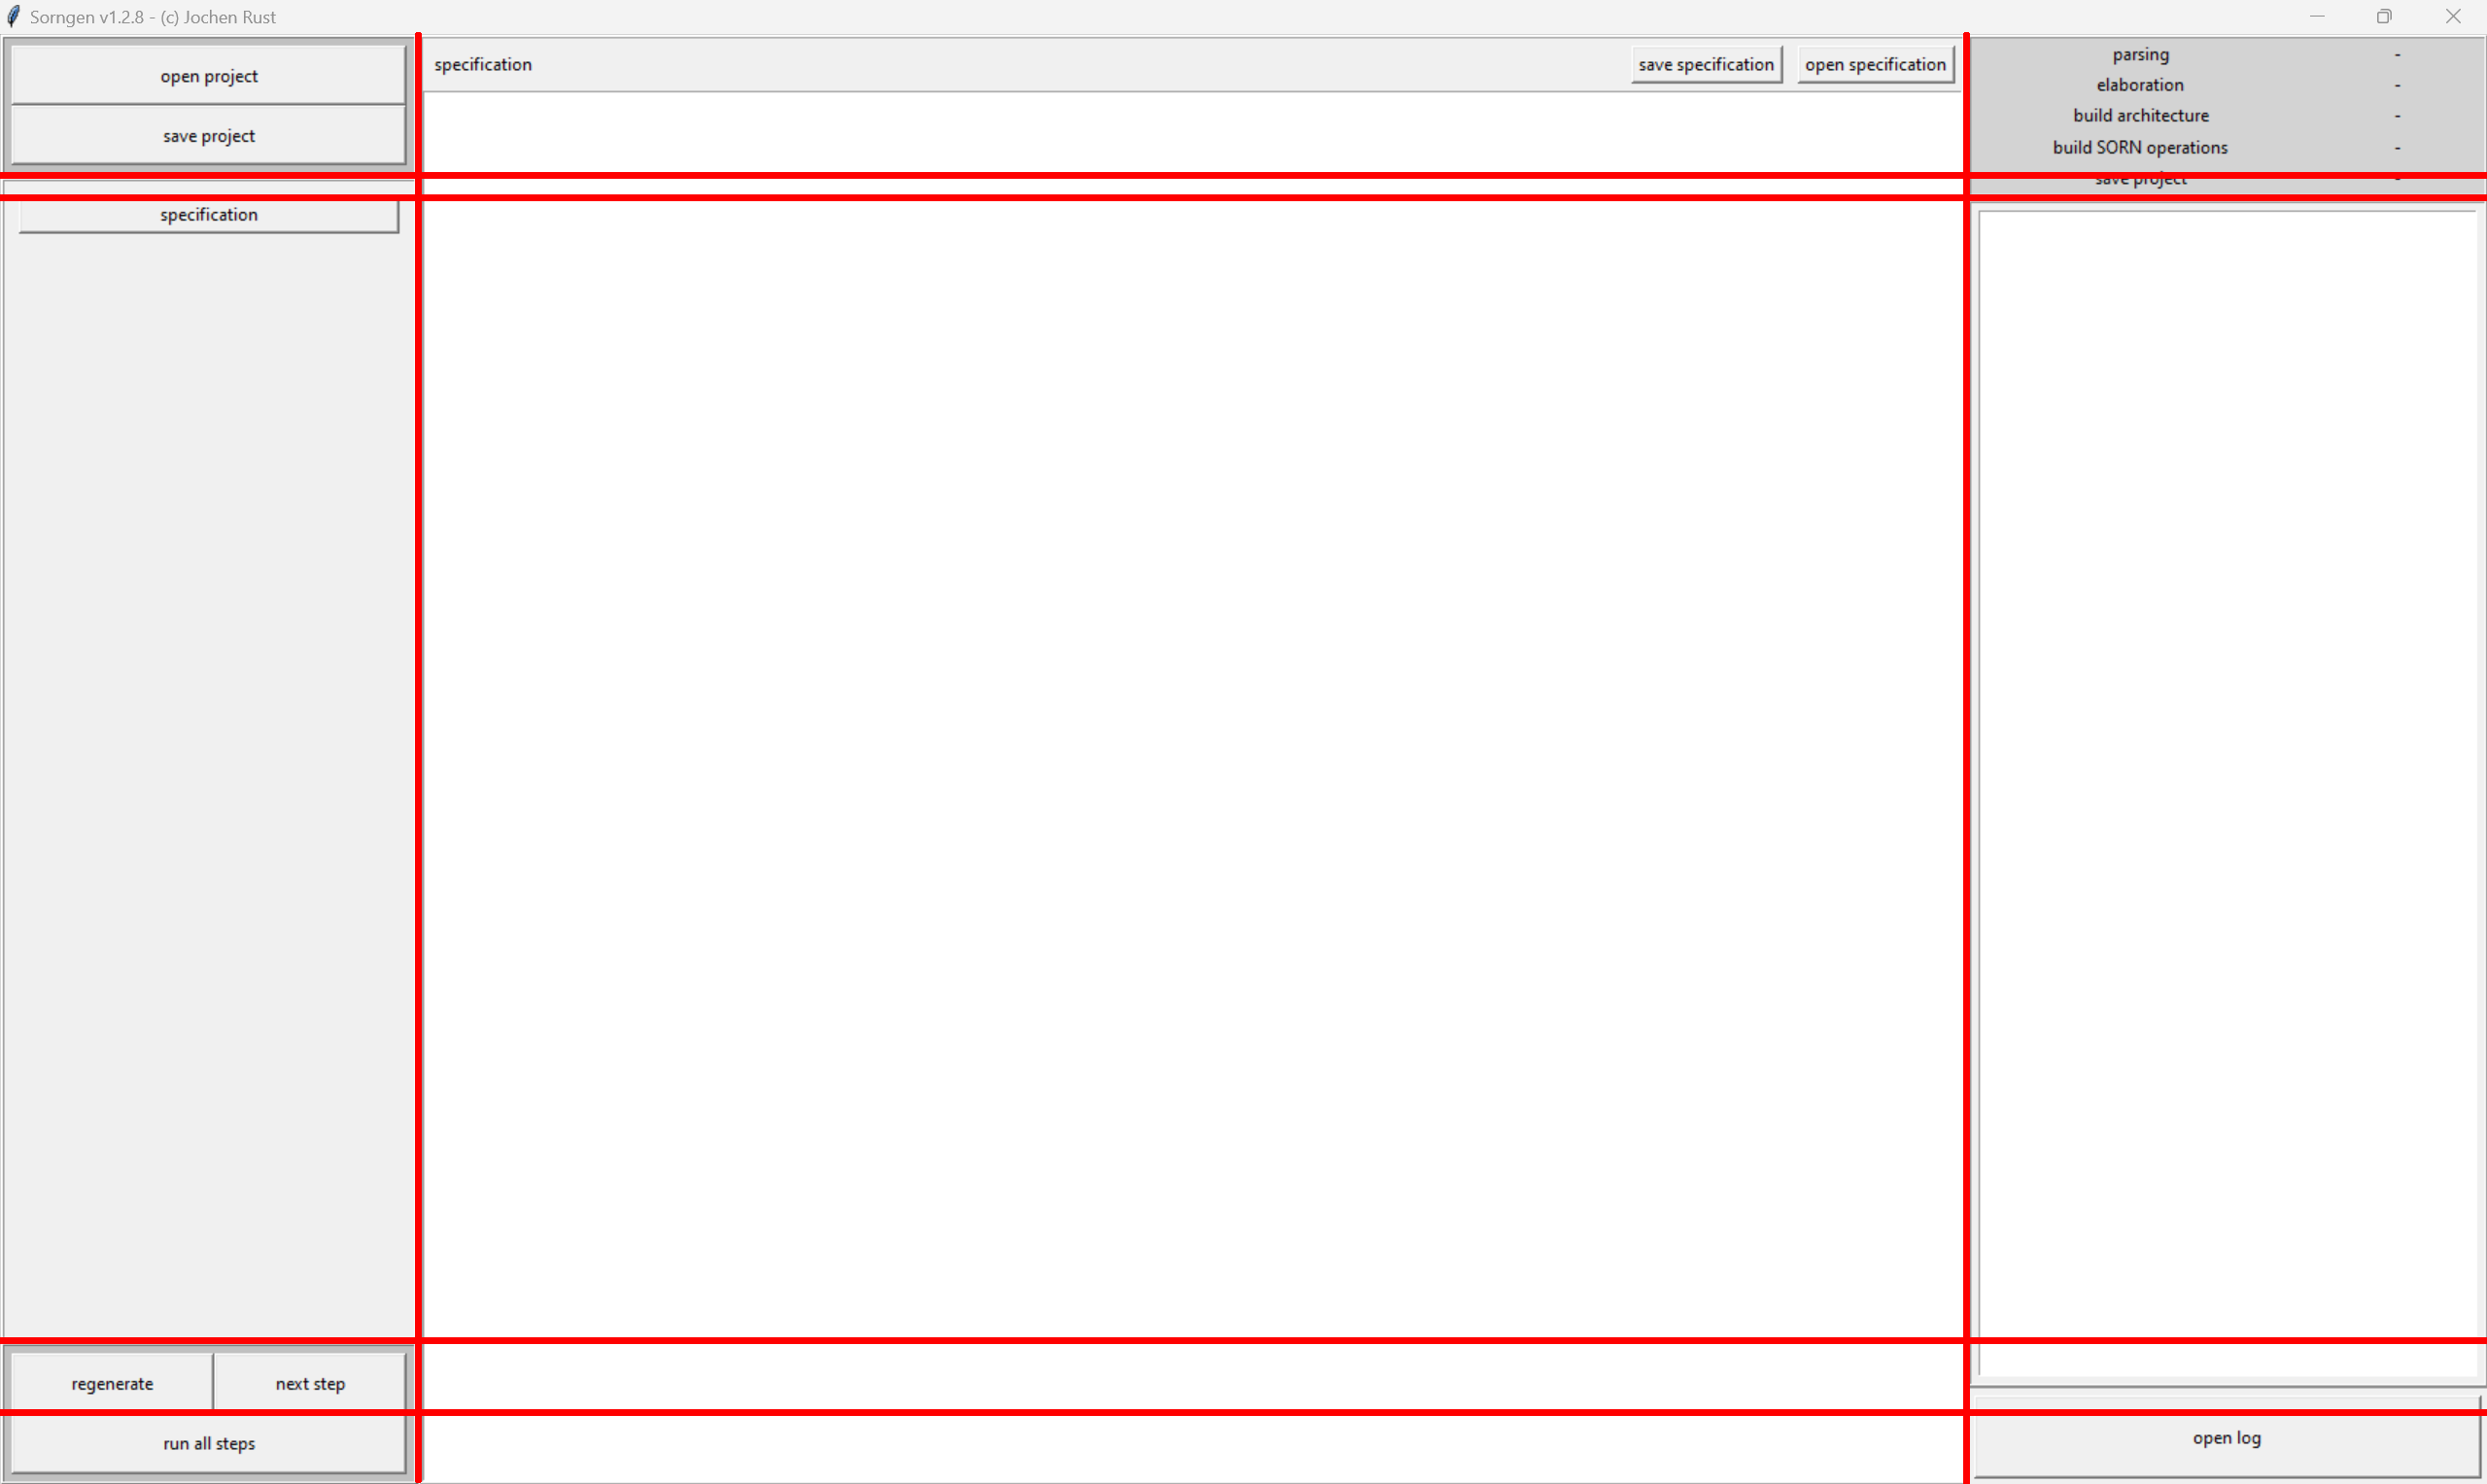
\includegraphics[width=0.75\linewidth]{root_layout.png}
    \caption{The root window layout. The red lines show columns and rows}
    \label{fig:root_layout}
\end{figure}
\begin{figure}[h]
    \centering
    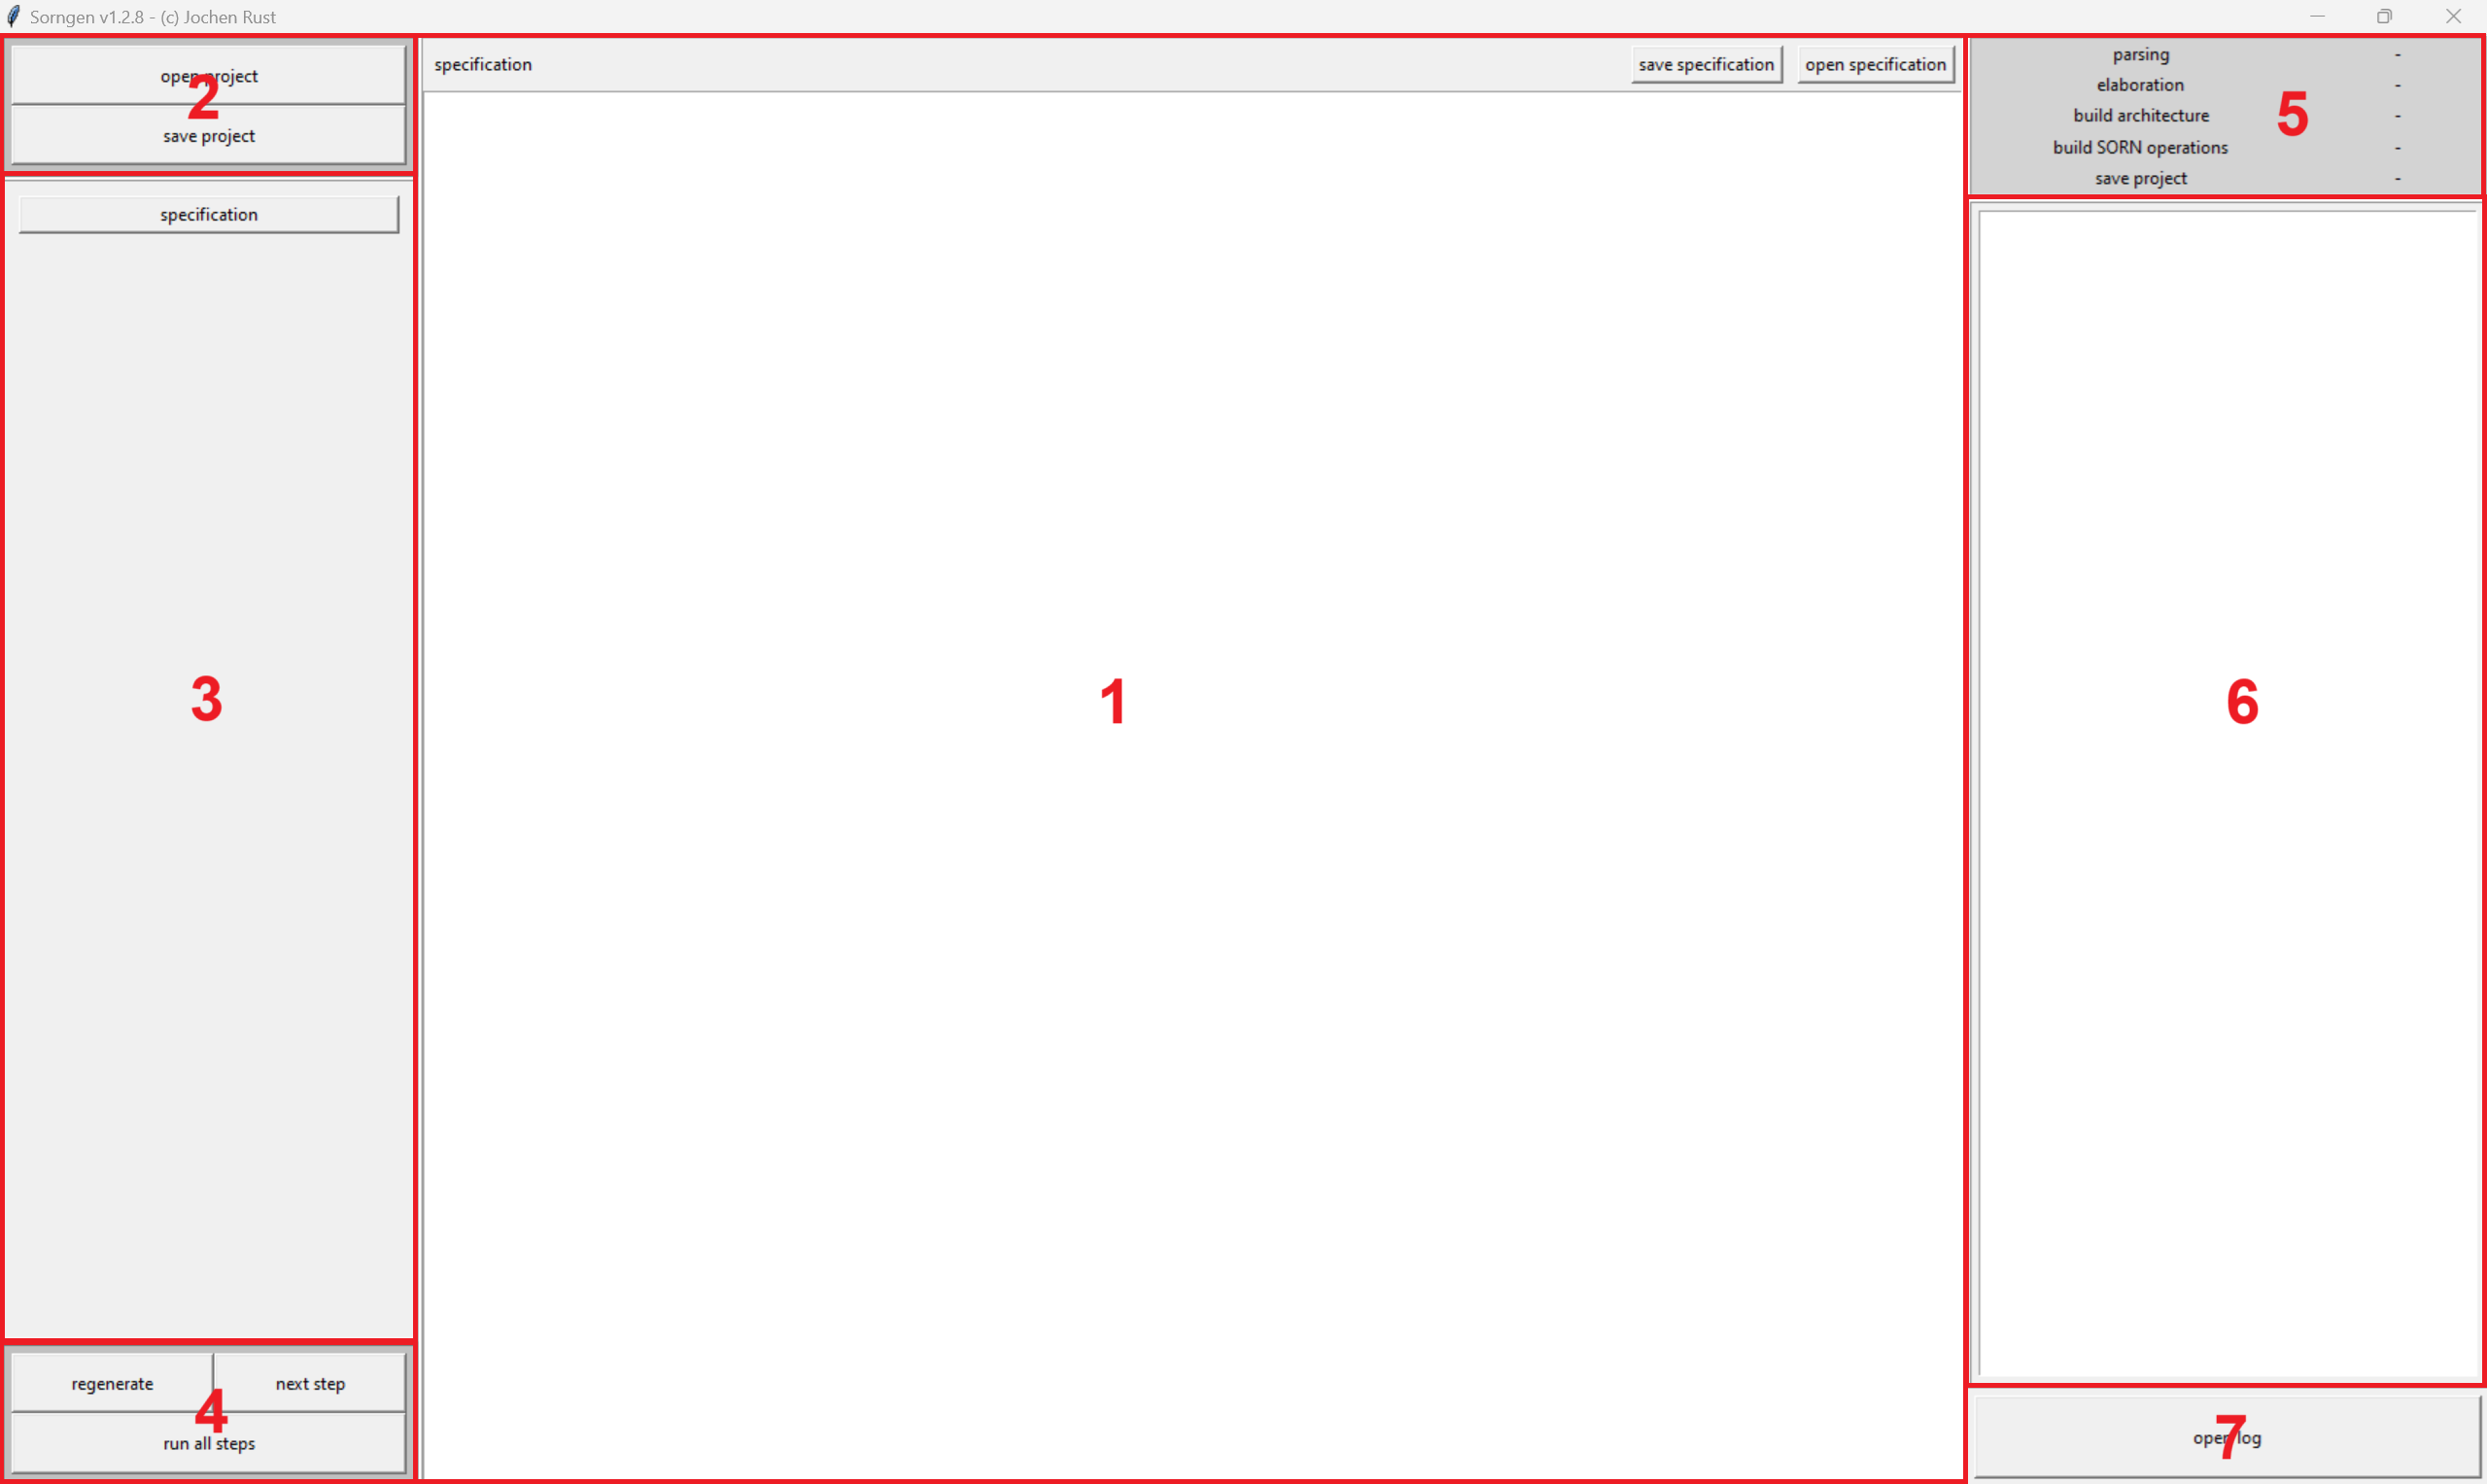
\includegraphics[width=0.75\linewidth]{root_map.png}
    \caption{The root Map. See \ref{enum:root_map} for legend}
    \label{fig:root_map}
\end{figure}

\end{document}
